\documentclass[12pt,english,brazil,a4paper,utf8,oneside]{utfpr-tcc}

% Este comando não é necessário: utilizei apenas para deixar o latex2rtf
% feliz (e descobrir a codificação do texto).
\usepackage[utf8]{inputenc}

% Suporte a figuras e subfiguras
\usepackage{graphics}
\usepackage{subfigure}

% Suporte a tabelas (principalmente do cronograma)
\usepackage{tabularx}
\usepackage{multirow}
\usepackage{array}
\usepackage{tabularx}
\usepackage{colortbl}
\usepackage{hhline}
\usepackage{xcolor}
\usepackage{indentfirst}

% Elementos geralmente utilizados na tabela do cronograma
\newcommand{\fullcell}{\multicolumn{1}{>{\columncolor[gray]{0.5}}c}{}}
\newcommand{\fullcellline}{\multicolumn{1}{>{\columncolor[gray]{0.5}}c|}{}}
\newcommand{\mc}[3]{\multicolumn{#1}{#2}{#3}}
\newcommand{\y}{\rule{8pt}{4pt}}
\newcommand{\n}{\hspace*{8pt}} 

% Define o caminho das figuras
\graphicspath{{images/}}

% Dados do curso que não precisam de alteração
\university{Universidade Tecnológica Federal do Paraná}
\universityen{Federal University of Technology -- Paraná}
\universityunit{Departamento Acadêmico de Computação}
\address{Campo Mourão}
\addressen{Campo Mourão, PR, Brazil}
\documenttype{Monografia}
\documenttypeen{Monograph}
\degreetype{Graduação}


%%%%%%%%%%%%%%%%%%%%%%%%%%%%%%%%%%%%%%%%%%%%%%%%%%%%%%%%%%%%%%%%%%%%%%%%%%%%%
% Alterar daqui para baixo
%%%%%%%%%%%%%%%%%%%%%%%%%%%%%%%%%%%%%%%%%%%%%%%%%%%%%%%%%%%%%%%%%%%%%%%%%%%%%

% Dados do curso. Caso seja BCC:
\program{Curso de Bacharelado em Ciência da Computação}
\programen{Undergradute Program in Computer Science}
\degree{Bacharel}
\degreearea{Ciência da Computação}
% Caso seja TSI:
% \program{Curso Superior de Tecnologia em Sistemas para Internet}
% \programen{Undergradute Program in Tecnology for Internet Systems}
% \degree{Tecnólogo}
% \degreearea{Tecnologia em Sistemas para Internet}


% Dados da disciplina. Escolha uma das opções e a descomente:
% TCC1:
\goal{Proposta de Trabalho de Conclusão de Curso de Graduação}
\course{Trabalho de Conclusão de Curso 1}
% TCC2:
% \goal{Trabalho de Conclusão de Curso de graduação}
% \course{Trabalho de Conclusão de Curso 2}


% Dados do TCC (precisa alterar)
\author{Gustavo Correia Gonzalez}  % Seu nome
\title{Um estudo sobre o uso do mecanismo de dicas personalizadas no ensino de conceitos básicos de programação} % Título do trabalho
\titleen{} % Título traduzido para inglês
\advisor{Prof. Dr. Igor Scaliante Wiese} % Nome do orientador. Lembre-se de prefixar com "Prof. Dr.", "Profª. Drª.", "Prof. Me." ou "Profª. Me."}
\coadvisor{Prof. Dr. Marco Aurélio Graciotto Silva} % Nome do coorientador, caso exista. Caso não exista, comente a linha.
\depositshortdate{2016} % Ano em que depositou este documento

% Dados da ficha catalografica. Ela é opcional, mas é uma boa ideia inserí-la. Exemplos para geração (http://fichacatalografica.sibi.ufrj.br/)
\fichacatautor{Gonzalez, Gustavo}  % Nome conforme citado (ou seja, no formato "Sobrenome, Nome").
\fichacatbib{Biblioteca da UTFPR de Campo Mourão} % Não alterar
\fichacatpum{M488} % Código Cutter-Sanborn. Use a primeira letra do sobrenome seguido do número conforme as primeiras letras do sobrenome e a tabela http://www.amormino.com.br/cutter-sanborn/cutter1.html
\fichacatpalcha{} % Assuntos do trabalho. Cada item deve ser enumerado e separado por ponto: 1. xxx. 2. yyy. 3. zzz.
\fichacatpdois{} % Deixar em branco


\begin{document}
	
\frontmatter
\maketitle

\begin{resumo}
% TODO: se possível, escreva um resumo estruturado. Para TCC 1, o resumo estruturado teria os seguintes elementos:

O elevado nível de reprovação em disciplinas onde são ensinados conceitos básicos de programação, em qualquer grau de ensino, é um problema enfrentado por muitos alunos e tem sido alvo de variadas pesquisas \cite{Holcomb:2016:RCA:2839509.2851062}. Existe um conjunto de razões que estão relacionadas com a origem do problema, como o método de ensino e aprendizagem, a falta de algumas competências e interesse por parte dos alunos, e a própria dificuldade do tema \cite{Sinclair:2015:MSE:2729094.2742586}.

\textbf{Contexto:} O desenvolvimento do estudo será realizado na Universidade Tecnológica Federal do Paraná, com alunos selecionados entre o primeiro ao oitavo semestre.

\textbf{Objetivo:} Avaliar o impacto do uso do mecanismo de dicas personalizadas no ensino de conceitos básicos de programação, mais especificamente em estrutura de condição e laço de repetição. Para atingir esse objetivo, foram criadas duas questões de pesquisas descritas como:

\begin{itemize}
	\item \textbf{QP}\textsubscript{1}: 
	\textit{Existe impacto do uso do mecanismo de dicas para minimizar erros e melhorar soluções de exercícios?}
	
	Esta questão de pesquisa tem como objetivo investigar se o mecanismo de dicas irá ajudar os alunos a obterem melhores resultados na execução de exercícios de programação. 
	
	\item \textbf{QP}\textsubscript{2}: 
	\textit{Quais dicas personalizadas ajudam mais os alunos?}
	
	Esta questão de pesquisa avaliará qual tipo de dica é melhor, podendo ser aleatorizadas em função do tipo do exercício, geradas a partir de erros cometidos em exercícios passados e sem dicas. Levando em consideração a fonte da dica gerada, podendo ser por alunos iniciantes, alunos experientes ou professores.
	
\end{itemize}

\textbf{Método:} Será desenvolvido um software para auxiliar o aprendizado de programação que utiliza um sistema de dicas personalizadas aos alunos no momento da realização de exercícios. Para avaliar o mecanismo de dicas será realizado um estudo controlado com três grupos de alunos distribuídos de forma homogênea em relação ao nível de conhecimento em programação. O primeiro grupo receberá dicas classificadas a partir de erros anteriores, o segundo será com dicas aleatorizadas levando em consideração o assunto abordado no exercício e o terceiro grupo não utilizará o mecanismo de dicas. Assim, os voluntário realizaram uma lista de exercícios e em cada subimissão ao sistema de dicas será gravado um \foreign{log} com dados que irão mensurar o desenpenho de cada voluntário, assim será realizado o estudo desses dados para responder as questões de pesquisa.

\textbf{Resultados esperados:} Espera-se que o software ajude no aprendizado dos alunos tornando o ensino de programação mais dinâmico e personalizado. Deste modo, espera-se diminuir o número de reprovações nas matérias introdutórias de programação e em desistências do curso de Ciência da Computação.
% ou, para TCC 2:
% \textbf{Contexto:} \\
% \textbf{Objetivo:} \\
% \textbf{Método:} \\
% \textbf{Resultados:} \\
% \textbf{Conclusões:}

% Palavras-chaves, separadas por ponto (tente não definir mais do que cinco)
\palavraschaves{Sistema, Mecanismo, Dicas, Dicas Personalizadas, Learnersourcing, Crowdsourcing}
\end{resumo}



% Caso seja TCC 2, precisa traduzir o resumo e as palavras-chaves para inglês:
% \begin{abstract}
% \textbf{Context:}
% \textbf{Objective:}
% \textbf{Method:}
% \textbf{Results:}
% \textbf{Conclusions:}

% Palavras-chaves em inglês, separadas por ponto.
% \keywords{}
% \end{abstract}



% Listas (opcionais, mas recomenda-se a partir de 5 elementos)
\listoffigures
\listoftables

% Sumário
\tableofcontents

\mainmatter
% TODO: incluir arquivos latex com os capítulos
\chapter{Introdução}

- terceira pessoa do singular - sujeito oculto

O ensino de linguagens de programação tem o propósito de conseguir desenvolver nos aluno um conjunto de competências necessárias para conceber programas e sistemas computacionais capazes de resolver problemas reais. O insucesso na aprovação dos estudantes em disciplinas de programação, é um tema que tem sido alvo de alguns estudos \cite{bosse2015reprovaccoes}, \cite{Cukierman:2015:PSU:2729094.2742623}.

O problema do insucesso é evidenciado por \citeonline{lahtinen2005study} realizaram uma pesquisa com 559 alunos e 34 professores de diferentes universidades para estudar as dificuldades na aprendizagem de programação. Como resultado foi percebido que as questões mais difíceis na programação são: a compreensão de como projetar um programa para resolver uma tarefa determinada, dividir as funcionalidades em procedimentos e encontrar erros de seus próprios programas. Estas são as capacidades que o aluno deve obter para entender as maiores entidades do programa em vez de apenas alguns detalhes sobre eles. Já os conceitos de programação mais difíceis foram recursão, ponteiros e referências, tipos de dados abstratos, manipulação de erro.

Com a necessidade de prover um suporte personalizado aos alunos, \citeonline{Elkherj:2014:SSR:2556325.2567864} criaram um sistema de dicas que permite o professore enviar uma dica personalizada em tempo real após verificar que o aluno realizou várias tentativas para resolver o exercício. Entretanto, com o aumento do número de alunos utilizando o sistema, os professores não conseguem oferecem um suporte a todos os alunos, assim utilização desse tipo de abordagem na construção do sistema de dicas apresenta limitações em relação a quantidade de alunos realizando os exercícios.

Nós utilizamos a abordagem do \foreign{learnersourcing} com o intuito de que os alunos, através de sua própria experiência resolvendo exercícios, podem criar dicas úteis através de suas implementações ou \foreign{bugs} que resolvem. Estes alunos podem então gerar sugestões para colegas com base em sua própria perícia. Mostraremos que, dada essa escolha de \foreign{design}, os alunos podem criar dicas que podem até mesmo substituir a assistência personalizada dos professores, quando essa assistência não está disponível.

O objetivo desse trabalho é criar um software de código aberto para auxiliar na aprendizagem de conceitos básicos de programação, implementando um sistema colaborativo de dicas escritas pelos próprios usuários. Para investigar se o uso do mecanismo de dicas personalizadas é capaz de melhorar o rendimentos dos alunos nos exercícios de estrutura de condição e laço de repetição, nós iremos aplicar um experimento controlado com três grupos distintos de alunos. O primeiro grupo utilizará o mecanismo de dicas normal que consiste em prover dicas de acordo com o exercício que o aluno está realizando. O segundo grupo utilizará o mecanismo de dicas personalizado que disponibiliza dicas de acordo com o exercício e o erro cometido na submissão. Por fim, o terceiro grupo utilizará o sistema sem o mecanismo de dicas.

No software serão implementadas funcionalidades que permitam o usuário resolver exercícios nas linguagens de programações C, C++ e Java, fornecer dicas para a solução de exercícios, um diário para relatar as dificuldades enfrentadas durante a execução dos exercícios. Estas informações são utéis e podem ser personalizar e melhorar o ensino de programação.

Para realizar a validação da ferramenta será realizado um estudo controlado na Universidade Tecnológica Federal do Paraná com três grupos de estudantes escolhidos aleatóriamente de forma homogênea em relação ao nível de conhecimento em programação. Com o experimento será possível avaliar se o grupo de alunos com dicas tem melhor desempenho que alunos sem o suporte do mecanismo. O desempenho será medido por: tempo, número de tentativas até a solução correta, qualidade do código gerado medida complexidade ciclimática do código, número de linhas entre as tentativas e tamanho da solução. Por fim também serão avaliadas se a qualidade das dicas são diretamente influenciadas com o nível de conhecimento do aluno, e se as dicas de alunos são melhores ou não em relação as dicas dos professores.

Os próximos capítulos estão organizados em três partes. O objetivo do capítulo de referencial teórico é apresentar e discutir os principais conceitos que envolvem este trabalho. Este  procedimento é importante, pois discutiremos os pontos de vista de diversos autores, assim como diversas abordagens alternativas. O objetivo do capítulo de proposta é apresentar a metodologia que será utilizada para desenvolver o estudo e o software. O objetivo do capítulo de resultados preliminares é apresentar os avanços que o estudo obteve durante o seu desenvolvimento.
\chapter{Referencial Teórico}

Neste capítulo apresentaremos uma revisão da literatura agrupando trabalhos relacionados a reprovações e dificuldades de alunos em disciplinas de programação, novas abordagens de ensino, sistemas de dicas. 

\section{Reprovações em Disciplinas de Programação}

O entendimento e aplicação dos conceitos estudados em disciplinas de programação é fundamental para que o aluno consiga desenvolver programas mais complexo. \citeonline{Helminen:2010:JPV:1879211.1879234} afirmam que a programação é uma competência essencial no curso de Ciência da Computação. Segundo \citeonline{bosse2015reprovaccoes} os estudantes normalmente apresentam uma grande dificuldade com os conteúdos abordados, ocasionando em reprovação ou desistência.


% TODO: Completar com os dados do estudo
\citeonline{Sinclair:2015:MSE:2729094.2742586} agruparam pesquisas internacionais como a \textit{National Survey of Student Engagement} (NSSE) feita na América do Norte e Canadá, a pesquisa \textit{Nacional Universidade Experience} (UES) e a pesquisa \textit{Survey Student Participation} (SES) que realizam a medida dos esforços dos alunos em atividades associadas com a aprendizagem efetiva. Esse estudo reúne dados relacionadas à Ciência da Computação sendo que os resultados desta meta-análise indicam que o curso de Ciência da Computação apresenta taxas mais baixas do que a média em muitos dos principais pontos de referência de engajamento.

\section{Mecanismo de Dicas}

% TODO: Começar pelas definições: O que são dicas? O que é um sistema de dicas?

Nas abordagens citadas a baixo, uma dica equivale a um auxílio ao aluno para que ele consiga realizar um exercício que esteja com dificuldade, essa dica pode ser oferecida tanto pelo professor ou colega de turma. Um sistema que utiliza esse conceito pode ser chamado de sistema de dicas, onde reproduz esse contato que o aluno teria com uma pessoa mais instruída quando precisa tirar uma dúvida ou pedir uma dica para realizar o exercício. Mas o aluno com dificuldades não pode ter esse apoio todo o tempo, então estão sendo criados sistema de dicas para suprir essa necessidade de auxiliar o aluno no seu aprendizado. 


% TODO: Conversar com o Igor
\citeonline{Elkherj:2014:SSR:2556325.2567864} apontam que as sugestões utilizadas em sistemas de aprendizagem on-line para ajudar os alunos quando eles estão tendo dificuldades são fixados antes do tempo e não dependem das tentativas mal sucedidas que o aluno já fez. Isto limita severamente a eficácia das sugestões. Eles desenvolveram um sistema alternativo para dar dicas aos estudantes. A principal diferença é que o sistema permite um instrutor enviar uma dica para um estudante após o aluno ter feito várias tentativas para resolver o problema e falhou. Depois de analisar os erros do aluno, o instrutor é mais capaz de entender o problema no pensamento do aluno e enviar-lhes uma dica mais útil. O sistema foi implantado em um curso de probabilidade e estatística com 176 alunos, obtendo \textit{feedback} dos alunos muito positivo. Mas o desafio que os autores enfrentam é como escalar efetivamente o sistema de forma que todos os alunos que precisam de ajuda obtenham dicas eficazes. Pois com uma grande quantidade de alunos ficaria exaustivo para os instrutores avaliarem cada submissão dos exercícios de cada aluno para retornarem uma dica especifica do erro cometido. Então eles criaram um banco de dados de dica que permite que os instrutores reutilizem, compartilhem e melhorem em cima de sugestões escritas anteriormente.

\citeonline{Price:2015:IIF:2787622.2787748} está utilizando um sistema de tutores inteligentes (STI) que podem manter os alunos no caminho certo, na ausência de instrutores, fornecendo sugestões e advertências para os alunos que precisam de ajuda. Além disso, as técnicas baseadas em dados podem gerar feedback automaticamente a partir de tentativas de resolução de um problema. O autor está aplicando o seu estudo permitindo que os alunos escrevam códigos que se conectam com seus interesses, tais como jogos, aplicações e histórias. Como exemplo concreto, imagine um aluno que esteja desenvolvendo um jogo simple, quer requer a utilização de variáveis, laços de repetição, condicionais. Mas o aluno está com dificuldades em relação a uma funcionalidade que o jogo terá, ele poderá pedir uma dica para implementar essa funcionalidade que será gerada automaticamente pelo sistema com relação as tentativas anteriores de outros alunos.

\citeonline{Cummins:2016:IUH:2876034.2893379} investigaram  o uso de dicas para 4.652 usuários qualificados em um ambiente de aprendizagem on-line de grande escala chamado Isaac, que permite aos usuários para responder a perguntas de física com até cinco dicas. Foi investigado o comportamento do usuário ao usar dicas, engajamento dos usuários com desvanecimento (o processo de tornar-se gradualmente menos dependentes das dicas fornecidas), e estratégias de dicas incluindo decomposição, correção, verificação ou comparação. Como resultados obtidos, os alunos apresentaram estratégias para as resoluções dos exercícios sendo a mais comum é ver o conceito da dica para realizar a decomposição do problema e, em seguida, enviar uma resposta correta. A outra estratégia é usar os conceitos da dica para determinar se a pergunta pode ser respondida, uma grande proporção dos usuários que utilizaram essa estratégia acabou não tentando responder a pergunta


%- fazer um resumo das abordagens de ensino e o engajamento dos estudantes
%\section{Abrodagens de ensino gerazaooo}
- reprovações em matérias de programação

- abordagem de ensino
	- tecnicas novas
	- dicas
	
- consideraçoes finais 
	- juntar tudo e falar o porque do meu tcc

%criar um capitulo de sumarização dos artigos relacionados e comentar o porque de usar o sistema de dicas que vou criar.
\chapter{Proposta}

Neste capítulo apresenta o método utilizado para a elaboração deste trabalho. A Figura \ref{figura:visaometodo} ilustra cada etapa a ser realizada para o desenvolvimento da abordagem proposta.

\begin{figure}[h]
	\captionsetup{justification=centering}
	\includegraphics[width=\linewidth]{visaogeraldometodoproposto.png}
	\caption{Visão geral do método proposto.}
	\label{figura:visaometodo}
\end{figure}

Para avaliar o impacto do uso do mecanismo de dicas personalizadas no ensino de conceitos básicos de programação, primeiramente será realizado a implementação do sistema de dicas utilizando o \foreign{framework} de desenvolvimento Laravel na versão 5.1. 

\section{Implementação do Mecanismo de Dicas}

Esta seção, descreve o sistema de dicas a ser desenvolvido. O processo de realização de exercícios, que é onde o sistema deve atuar, pode ser dividi do em quatro fases: cadastro do usuário, realização de exercícios, utilização de dicas (providas por usuários do sistema) e validação do exercício. A descrição apresentada será usada para a modelagem do sistema.

\begin{figure}[h]
	\captionsetup{justification=centering}
	\includegraphics[width=\linewidth]{sistemadicas.png}
	\caption{Visão geral do sistema de dicas.}
	\label{figura:sistemadicas}
\end{figure}

\subsection{Cadastro do Usuário}

Quando um usuário desejar realizar o cadastro no nosso sistema, ele poderá escolher entre a opção de aluno ou professor. O aluno, realiza exercícios disponíveis no banco de dados do sistema, preenche um diário não obrigatório para cada exercício, cria uma dica para cada exercício e consulta seu perfil com seus dados pessoais e um relatório de suas submissões de exercícios. O professor, além de realizar as mesmas atividades do aluno, também poderá criar salas com exercícios pré-definidos convidando alunos para fazer parte dela e submeter exercícios para o sistema.

\subsection{Cadastro de Exercícios}

Essa funcionalidade do sistema só poderá ser acessada se o usuário for um professor. Sendo assim, o professor terá que cadastrar um enunciado, qual linguagem é para ser utilizada na resolução, o nível (fácil, médio ou difícil), o tipo do exercício (condicional ou laço de repetição), a resposta que poderá ser escrita em um campo ou um \foreign{upload} do arquivo com as respostas. Cada exercício cadastrado será agregado a uma lista de exercícios que o professor irá criar antes de cadastrar os exercícios.


% TODO: Colocar formato de exemplo de uma resposta

\subsection{Cadastro de Turma}

O professor poderá realizar o cadastro de uma classe para adicionar seus alunos e passar as listas de exercícios e acompanhar o rendimento de cada aluno. Para cadastrar uma turma é necessário um nome da turma e um professor, com isso o professor poderá adicionar os alunos desejados.

\subsection{Realização de Exercícios}

Após a conclusão do cadastro de usuário, o aluno ou professor terão acesso as funcionalidades especificas de cada tipo de usuário. Dessa forma, o usuário poderá resolver uma lista de exercícios de duas formas: estando vinculado a uma turma ou individualmente. Caso o usuário esteja vinculado a uma turma, a lista de exercícios que ele poderá resolver será a que o professor responsável pela turma criou. Caso o usuário não faça parte de uma turma, ele terá que pesquisar por uma lista de exercícios informando qual assunto, estrutura de condição ou laço de repetição, ele deseja realizar. 

Depois que o usuário encontrar uma lista de exercícios, o sistema apresentará os exercícios à serem resolvidos na ordem em que foram adicionados na lista. Assim o usuário poderá trabalhar em sua solução e submeter ao sistema para correção utilizando a linguagem de programação escolhida pelo professor na criação da lista de exercícios, essa resolução poderá estar correta ou não. Se estiver correta, o sistema apresentará uma mensagem de parabenização e redirecionará o usuário para o próximo exercício. Caso a resolução estiver errada o sistema retornará qual o erro ocorrido na compilação, assim o usuário poderá realizar outras submissões até que consiga obter sucesso na resolução ou requisitar uma dica para o sistema para auxiliá-lo na construção da resposta. 

Cada submissão, tanto correta ou incorreta, é gravada no banco de dados na forma de \foreign{log}, sendo salvo os dados: a usuário que realizou o exercício, todas as submissões, os erros cometidos, o tempo demorado para obter sucesso no exercício, (ver a onde foi marcado no papel).


\subsubsection{Utilização das Dicas}

O usuário apenas poderá consultar uma dica caso o exercício enviado para validação não esteja correto e ele escolha a opção de disponibilização de dicas, assim ele terá direito a três dicas selecionadas aleatoriamente pelo mecanismo. O usuário irá escolher consultar uma das três dicas e após a consulta ele poderá realizar uma nova submissão do exercício.

\subsection{Cadastro de Dica}

O cadastro de uma dica pode ser realizado quando o usuário submete um exercício para validação e obtêm êxito, assim o sistema apresentará uma tela perguntando se o usuário deseja contribuir com uma dica, caso aceite, o sistema irá redirecionar o usuário para a tela onde será realizado o cadastro da dica, onde ele irá descrever em um campo a dica que deseja compartilhar. Também será apresentada a solução do mesmo exercício de outro usuário para que seja escrito uma dica. 

\subsection{Cadastro do Diário}

No processo de execução de um exercício o usuário poderá preencher um diário relatando suas experiências, essa funcionalidade será apresentada aos usuários caso o professor deseja receber o preenchimento do diário dos exercícios da lista. 

Caso o professor pretende receber os diários dos exercícios da lista de sua turma, o usuário após cada submissão da resolução no sistema produzirá um diário que será informado os dados referentes a experiência de realizar o exercício. 

\subsection{Boca (BOCA Online Contest Administrator)}

Para realizar a compilação dos exercícios no sistema de dicas, será utilizado funções do \foreign{software} BOCA \citeonline{de2004boca} que é escrito predominantemente em PHP, o que permitiria sua execução em qualquer plataforma compatível com tal linguagem. No entanto, o sistema de julgamento depende de scripts Bash e de funcionalidades específicas do sistema operacional Linux (isolamento de recursos/jail). O Boca é amplamente utilizado em maratonas de programação em todo o Brasil, são exemplos de maratonas: Maratona de Programação da USP, Maratona de Programação da FACENS, Maratona de Programação da Faculdade de Informática de Presidente Prudente e Copa de programação da PUC-SP. 

\section{Formato do Estudo}

Esta seção apresentará o formato do estudo, descrevendo como serão realizados o teste do sistema, a criação do banco de exercícios e banco de dicas e como serão respondidas as questões de pesquisa.

\subsection{Teste do sistema}

Após o desenvolvimento do sistema ser concluído. Antes de realizar os estudos, será necessário executar uma etapa de teste para encontrar possíveis erros no sistema. Para que essa etapa aconteça, será con. Rese vocado um grupo de alunos de forma voluntária para utilizarem as funcionalidades do sistema e reportar se existe algum erro no sistema. Os alunos deverão reportar os erros encontrados através de criação de \foreign{issues} no \foreign{GitHub} onde está o repositório do sistema. Todos os erros serão corrigidos antes de realizar os estudos para avaliar o sistema.

\subsection{Banco de Exercícios}

O banco de dados de exercícios será criado a partir de exercícios selecionados para diferir dos exercícios realizados na matéria de Algoritmos oferecida pelo curso, a seleção terá a finalidade de prevenir que o voluntário do estudo de avaliação do sistema já tenha realizado o exercício. Os exercícios serão divididos em três grupos, o primeiro abordará conceitos básicos da linguagem de programação como entrada e saída de dados, declaração de variáveis e constantes, operações e funções matemáticas. O segundo grupo refere-se a estruturas condicionais e o terceiro grupo trata de estruturas de repetição.

\subsection{Banco de Dicas}

\begin{figure}[ht]
	\captionsetup{justification=centering}
	\includegraphics[width=\linewidth]{fluxo.png}
	\caption{Fluxos para criação de dicas.}
	\label{figura:dicafluxo}
\end{figure}


O banco de dicas será provido após a conclusão do banco de exercícios, assim será realizada uma convocação por formulário \textit{online} aos estudantes da Universidade Tecnológica Federal do Paraná do curso de Bacharelado em Ciência da Computação para se voluntariarem a utilizar o sistema de dicas por um determinado período em um dia que será estipulado no formulário. Os voluntários utilizaram o sistema de dicas em um ambiente controlado sendo esse um laboratório da Universidade Tecnológica Federal do Paraná com um professor ou alunos monitorando as atividades e tirando as possíveis dúvidas dos participantes. 

A criação das dicas conforme a Figura \ref{figura:dicafluxo} irá respeitar dois fluxos de execução, sendo eles: fluxo de reflexão e fluxo de comparação. Os dois fluxos são iniciados quando o usuário recebe uma lista de exercícios para ser realizada. Após o usuário ter uma lista de exercícios o fluxo de reflexão começa, o sistema irá apresentar um exercício da lista para ser resolvido e o usuário poderá começar a realizar a solução. Após a solução ser concluída, o usuário submete a solução para validação, o sistema irá executar a solução do exercício e verificar se está correta ou não. Caso a solução não estiver correta, o sistema redireciona para a etapa de realização de solução, nessa etapa o usuário poderá pedir uma dica para o sistema. Caso a solução estiver correta, o sistema irá redirecionar o usuário para a tela aonde ele criará a dica para o exercício e irá realizar o cadastro dela no banco de dicas.

Após o usuário gerar uma dica do exercício realizado, o sistema irá seguir o fluxo de comparação. Deste modo, o sistema irá procurar no banco de dados soluções de outros usuários do exercício realizado. O sistema irá apresentar ao usuário a pior e a melhor solução do exercício para que ele crie uma dica para melhorar as duas soluções. As dicas de otimização serão cadastradas no banco de dados de dicas para auxiliar outros usuários na resolução do exercício.

\subsection{Avaliação do Sistema de Dicas}

\begin{figure}[ht]
	\captionsetup{justification=centering}
	\includegraphics[width=\linewidth]{estudo.png}
	\caption{Visão geral da aplicação do estudo.}
	\label{figura:estudo}
\end{figure}

Nesta subseção será explicado as duas etapas que serão realizadas para responder as duas questões de pesquisa. A primeira etapa consiste em aplicar um estudo controlado na Universidade Tecnológica Federal do Paraná para gerar os dados de \foreign{log} de execução das listas de exercícios necessários. Dessa forma, após a geração dos dados de \foreign{log} a segunda etapa será inicializada. A segunda etapa apresenta as análises que serão feitas para responder as duas questões de pesquisa.

\begin{table}[]
	\centering
	\captionsetup{justification=centering}
	\caption{Formulário para aquisição de voluntários.}
	\label{tabela:formulário}
	\begin{tabular}{l}
		\hline
		Perguntas                        \\ \hline
		Nome?                            \\
		Idade?                           \\
		Telefone?                        \\
		Email?                           \\
		Curso?                           \\
		Tempo que está cursando o curso? \\
		Semestre?                        \\ \hline
	\end{tabular}
\end{table}

A Figura \ref{figura:estudo} representa a primeira etapa da avaliação do sistema, onde será necessário a colaboração de voluntários do curso de Bacharelado em Ciência da Computação para o experimento presencial que será realizado na Universidade Tecnológica Federal do Paraná, para isso será criado um formulário no \foreign{Google Forms} representado na Tabela \ref{tabela:formulário} e disponibilizado \foreign{online} para os alunos do curso.

Os voluntários serão divididos em três grupos distintos de acordo com o nível de conhecimento em programação, o nível de cada voluntário será estimado de acordo com o tempo que está na graduação e o semestre que se encontra. Os três grupos irão realizar os mesmos exercícios mas utilizaram funcionalidades diferentes do sistema,  

\begin{itemize}
	\item \textbf{Grupo 1}: utilizará o mecanismo de dicas que prove dicas de acordo com o exercício que o aluno está realizando.
	
	\item \textbf{Grupo 2}: utilizará o mecanismo de dicas personalizado que disponibiliza dicas de acordo com o exercício e o erro cometido na submissão.

	\item \textbf{Grupo 3}: utilizará o sistema sem o mecanismo de dicas.
\end{itemize}

Toda submissão realizada pelos três grupos de voluntários será gravada no \foreign{log} de submissões, sendo salvo os dados: a usuário que realizou o exercício, todas as submissões, os erros cometidos, o tempo demorado para obter sucesso no exercício. Após todos os voluntários tiverem finalizados todos os exercícios da lista, o estudo presencial será finalizado com a aplicação de um questionário representado na Tabela \ref{tabela:questionárioestudo} para avaliar a usabilidade do sistema e a experiência da utilização de um sistema \foreign{web} para solucionar exercícios de programação.

\begin{table}[]
	\centering
	\captionsetup{justification=centering}
	\caption{Questionário do estudo presencial.}
	\label{tabela:questionárioestudo}
	\begin{tabular}{l}
		\hline
		Perguntas                        \\ \hline
		pergunta1?                            \\
		pergunta2?                           \\
		pergunta3?                        \\
		pergunta4?                           \\
		pergunta5?                           \\
		pergunta6? \\
		pergunta7?                        \\ \hline
	\end{tabular}
\end{table}

A segunda etapa da avaliação do sistema responderá as duas questões de pesquisa, será analisado os dados do \foreign{log} de submissões realizados na primeira etapa. A primeira questão de pesquisa tem como objetivo investigar se o mecanismo de dicas irá ajudar os alunos a obterem melhores resultados na execução de exercícios de programação, essa questão será respondida a partir da avaliação do desempenho dos grupos que utilizaram o sistema com o mecanismo de dicas em relação ao grupo que utilizou o sistema sem o mecanismo, também será avaliado o questionário respondido pelos voluntários.   

A segunda questão: Quais dicas personalizadas ajudam mais os alunos? Será respondida com a análise da comparação do desempenho do primeiro grupo de voluntário com o segundo, e verificando se as dicas de voluntários mais experientes possuíram melhor avaliação em relação as dicas dos voluntários menos experientes.
\chapter{Resultados Preliminares}

Neste capítulo será apresentado os resultados premliminares, onde utilizamos o diagrama de caso de uso apresentado na Figura \ref{figura:sistemadicas} encontrada no Capítulo 3 para realizar o desenvolvimento do sistema no \foreign{framework} de desenvolvimento Laravel na versão 5.1.

Assim foi desenvolvido o registro de usuário, o login, a tela de resetar senha, o cadastro de professor e o cadastro de aluno representadas respectivamente nas figuras a seguir.

\begin{figure}[]
	\captionsetup{justification=centering}
	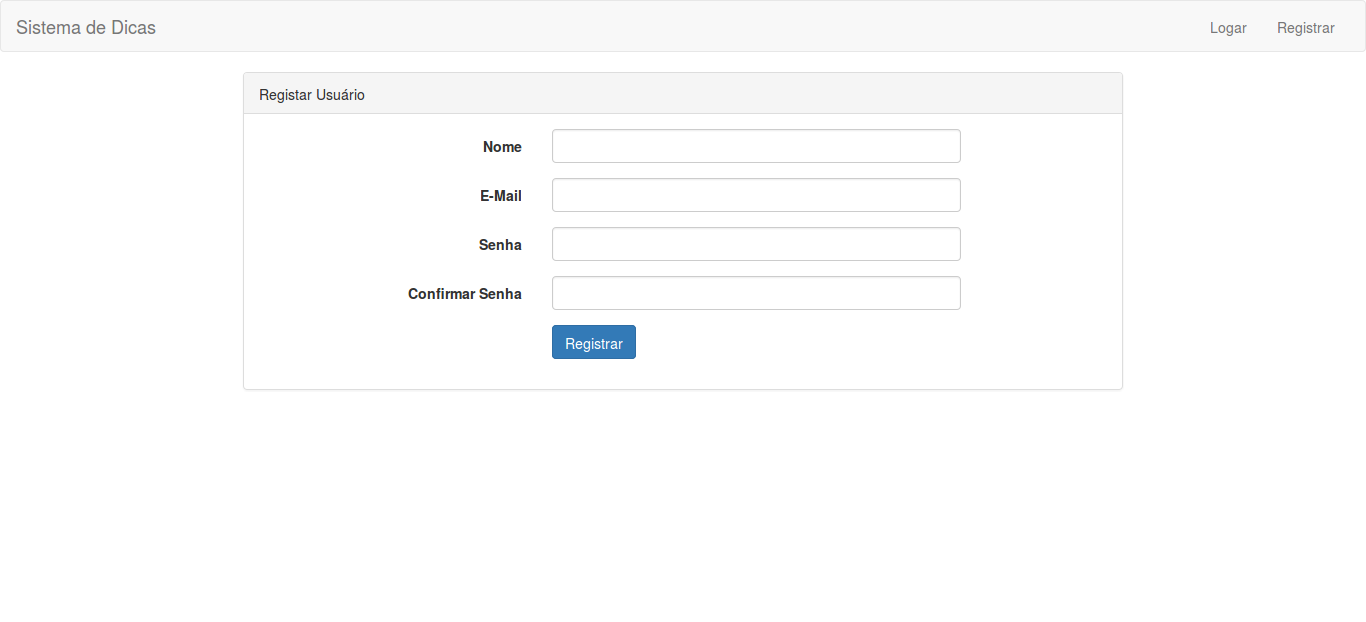
\includegraphics[width=\linewidth]{imagenssoftware/registrarusuario.png}
	\caption{Tela de regustro de usuário.}
	\label{figura:registrarusuario}
\end{figure}

\begin{figure}[h]
	\captionsetup{justification=centering}
	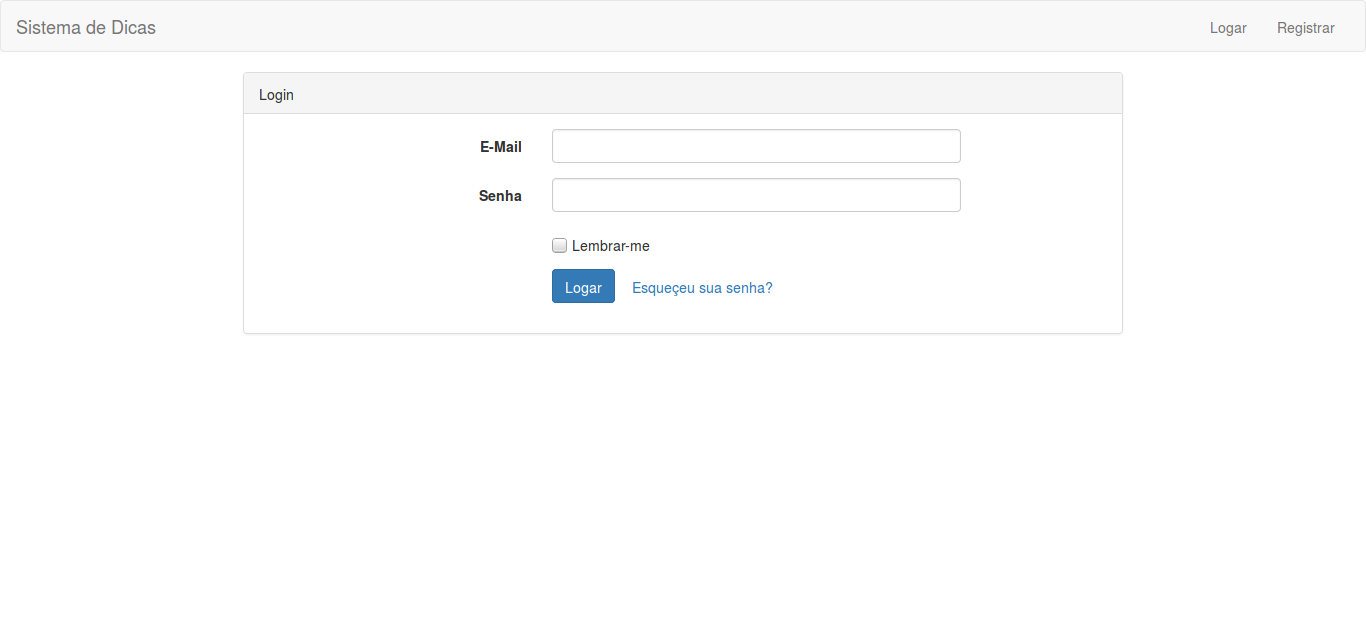
\includegraphics[width=\linewidth]{imagenssoftware/logar.png}
	\caption{Tela de login no sistema.}
	\label{figura:logar}
\end{figure}

\begin{figure}[h]
	\captionsetup{justification=centering}
	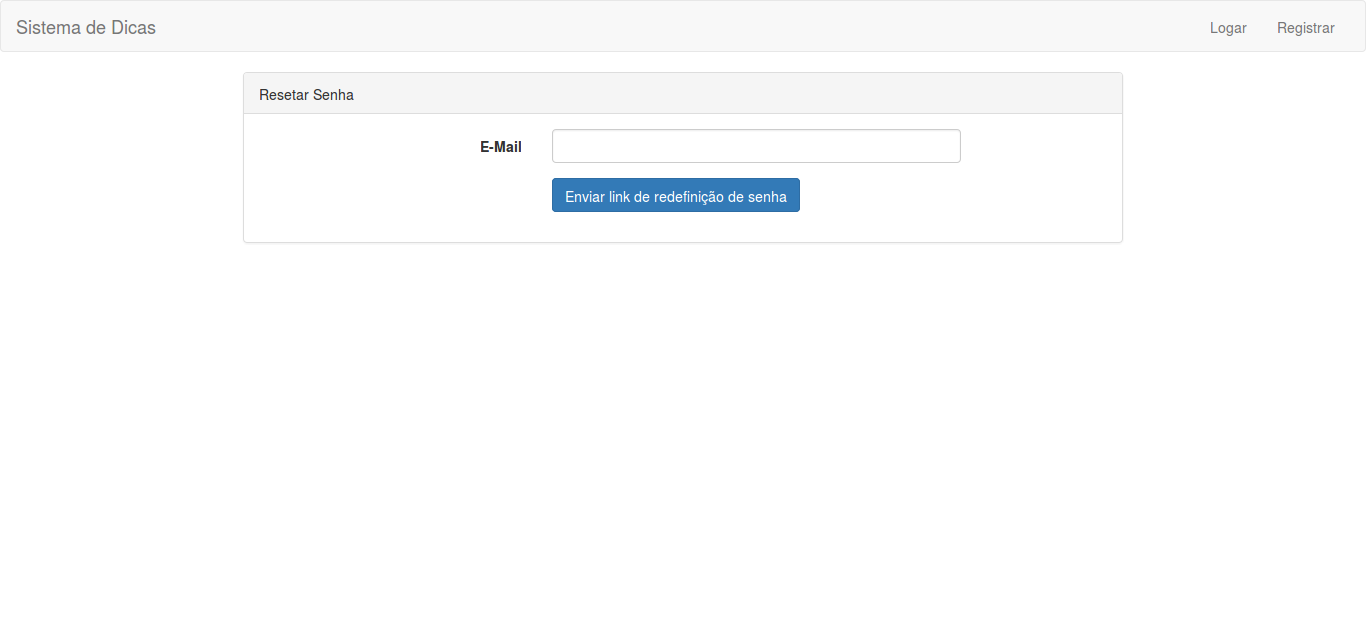
\includegraphics[width=\linewidth]{imagenssoftware/resetarsenha.png}
	\caption{Tela para resetar a senha.}
	\label{figura:resetarsenha}
\end{figure}

\begin{figure}[h]
	\captionsetup{justification=centering}
	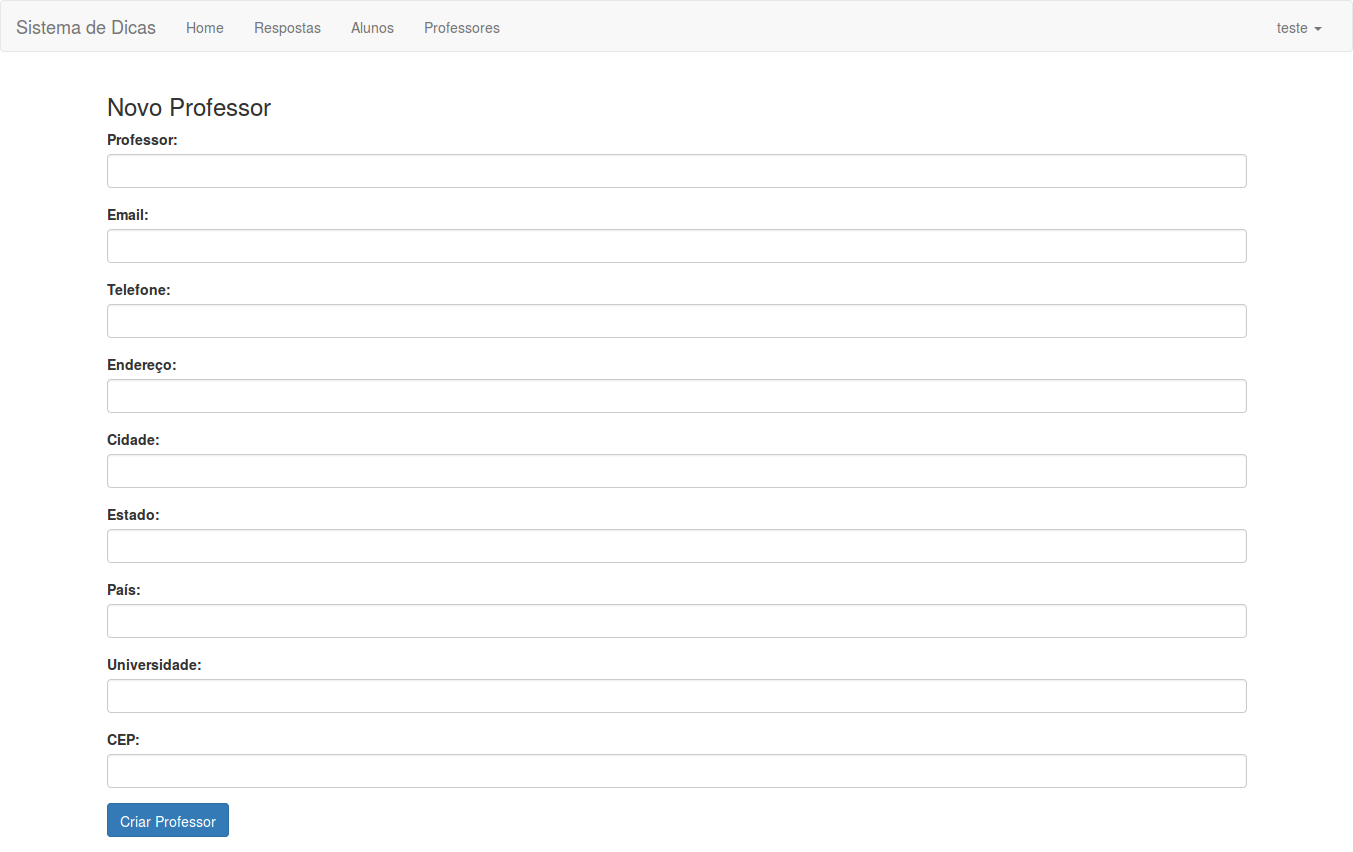
\includegraphics[width=\linewidth]{imagenssoftware/cadastroprofessor.png}
	\caption{Tela de cadastro de professor.}
	\label{figura:cadastroprofessor}
\end{figure}

\begin{figure}[h]
	\captionsetup{justification=centering}
	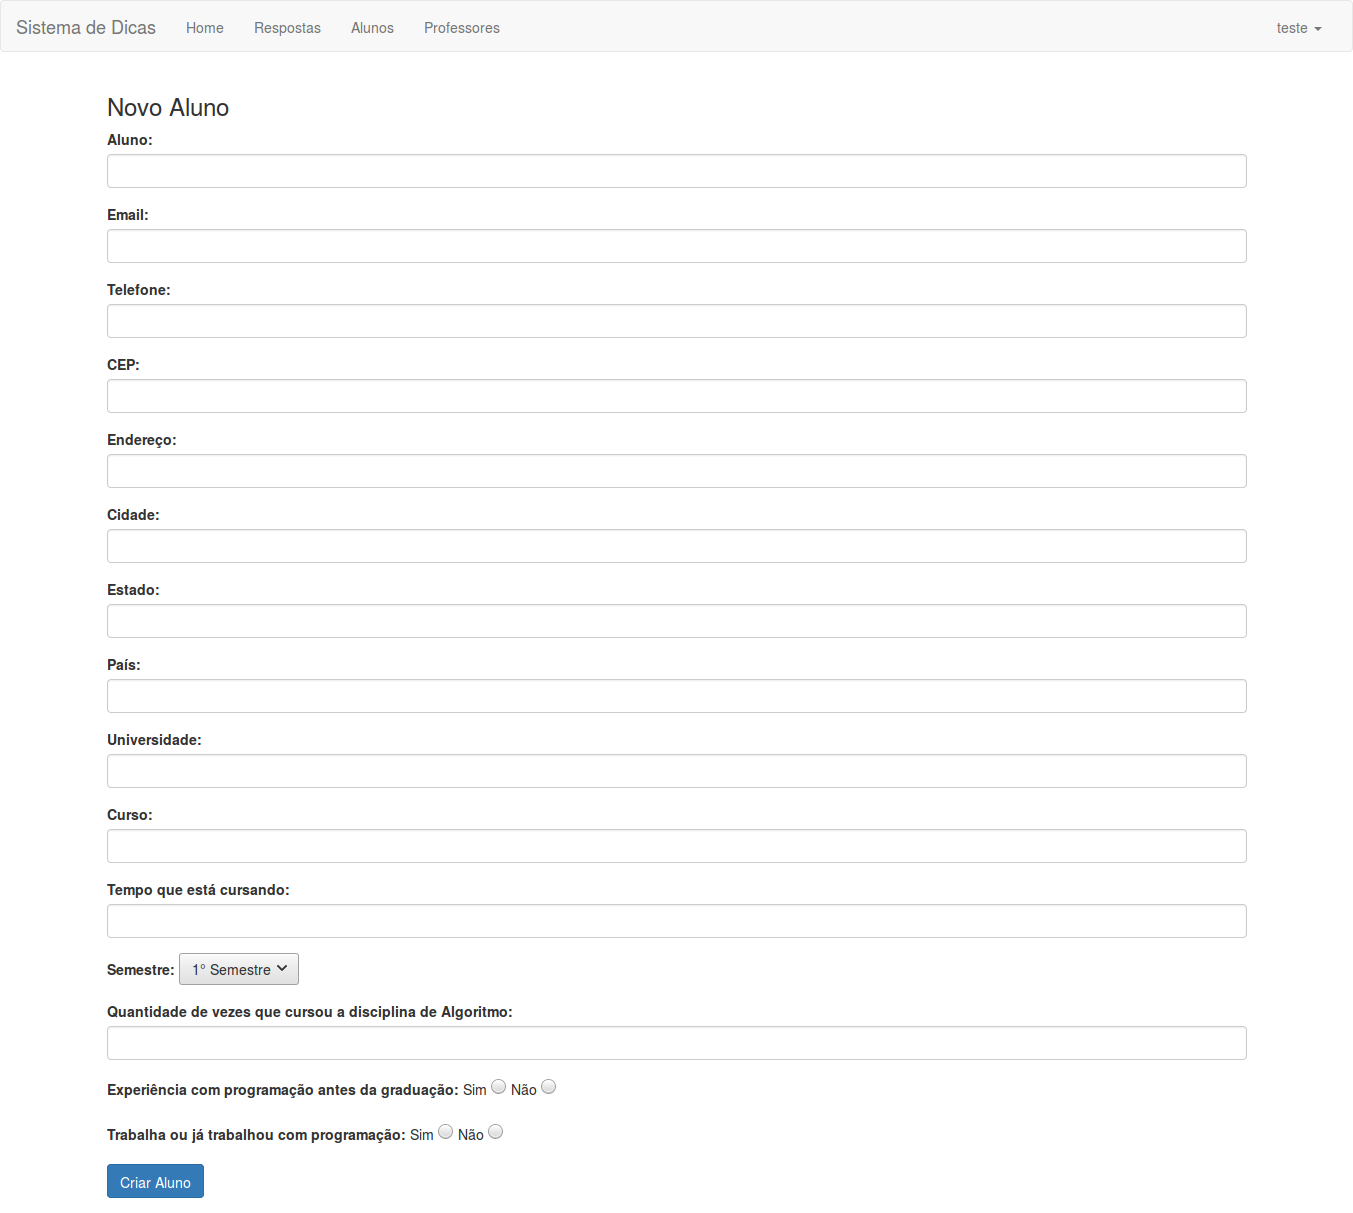
\includegraphics[width=\linewidth]{imagenssoftware/cadastroaluno.png}
	\caption{Tela de cadastro de aluno.}
	\label{figura:cadastroaluno}
\end{figure}
\chapter{Cronograma}

A \cref{tabela:cronograma} apresenta o cronograma das tarefas a serem realizadas futuramente.

\begin{table}[ht]
	\captionsetup{justification=centering}
	\caption{Cronograma}
	\label{tabela:cronograma}
	\begin{tabular}{|l|c|c|c|c|c|c|}
		\hline
		& Janeiro & Fevereiro & Março & Abril & Maio & Junho \\ \hline
		Implementação do Sistema 		& X       & X         &       &       &      &       \\ \hline
		Escrita do Trabalho      		&         & X         & X     & X     & X    & X     \\ \hline
		Teste do Sistema         		&         &           & X     &       &      &       \\ \hline
		Banco de Exercícios      		&         &           & X     &       &      &       \\ \hline
		Banco de Dicas           		&         &           &       & X     &      &       \\ \hline
		Avaliação do Sistema de Dicas   &         &           &       & X     & X    &       \\ \hline
		Defesa                     		&         &           &       &       &      & X     \\ \hline
	\end{tabular}
\end{table}

\bibliographystyle{abnt-alf}
\bibliography{main} % geração automática das referências a partir do arquivo main.bib

\backmatter
\end{document}
